\documentclass[12pt,a4paper]{article}

\usepackage{amsmath, amssymb, amsthm}
\usepackage{graphicx}
\usepackage{hyperref}
\usepackage[margin=1in]{geometry}
\usepackage{booktabs}
\usepackage{caption}
\usepackage{subcaption}

\title{On the Distribution of Primes Represented by $p^{2}+4q^{2}$ with $p,q$ Prime}

\author{NullLabTests \\ \texttt{github.com/NullLabTests/prime-number-research}}

\date{\today}

\begin{document}

\maketitle

\begin{abstract}
We present a systematic empirical investigation of primes of the form
$R = p^{2}+4q^{2}$ where both $p$ and $q$ are themselves prime.
Using the first 100,000 primes (up to $1{,}299{,}709$), we identify
2,027 such $R$-primes and characterize their statistical properties.
We report four principal findings: (i)~the relative density of
$R$-primes decays as a power law $C(B) \propto B^{0.79}$, yielding
roughly one $R$-prime per 640 primes at the million scale;
(ii)~every $R$-prime satisfies $R \equiv 1 \pmod{4}$, and remarkably
98\% satisfy $R \equiv 5 \pmod{8}$ --- a strong statistical bias
with no elementary explanation; (iii)~the gap distribution closely
follows the exponential model of Cram\'er, consistent with
randomness; and (iv)~unlike the full prime set, $R$-primes deviate
significantly from Benford's first-digit law
($\chi^{2}=177$, $p<10^{-15}$). We further show that a Random Forest
regressor with engineered features cannot outperform a constant
mean-guess for gap prediction, consistent with the hypothesis that
gaps behave as independent exponential random variables.
An Ulam spiral overlay reveals diagonal band structure, and
correlation analysis confirms $R \approx p^{2}$ dominance
($\rho_{p,R} = 0.87$). All data and code are open-source.
\end{abstract}

\section{Introduction}

Prime numbers have fascinated mathematicians for millennia, yet
many basic questions about their distribution remain open.
The study of primes representable by quadratic forms dates to
Fermat's theorem on sums of two squares: a prime $p$ can be
written as $p = x^{2}+y^{2}$ iff $p \equiv 1 \pmod{4}$.
Subsequent work generalized this to forms $x^{2}+ny^{2}$,
with complete characterizations known for many $n$ via class
field theory~\cite{cox2013primes}.

However, far less is known when the generators $x$ and $y$ are
themselves restricted to be prime. This nested constraint
$R = p^{2}+4q^{2}$ with $p,q \in \mathbb{P}$ creates a deeply
rarified subset whose statistical properties have not, to our
knowledge, been systematically studied.

In this paper we perform a computational census of
$R$-primes, analyzing their density, modular structure, gaps,
Benford behavior, and predictability via machine learning.
All code is available at
\url{https://github.com/NullLabTests/prime-number-research}.

\section{Data and Methodology}

We use the first 100,000 primes, up to $1{,}299{,}709$,
sourced from a standard reference table. Primality testing
for candidate values $R = p^{2}+4q^{2}$ uses $O(1)$ set
membership lookup against this pre-computed list.

For each pair of primes $(p,q)$ with $p \geq q$ (to avoid
symmetry), we compute $R = p^{2}+4q^{2}$ and test membership.
The $p \geq q$ convention avoids double-counting since the
form is symmetric in the sense that $p^{2}+4q^{2}$ is not
symmetric (unlike $p^{2}+q^{2}$), but the unordered pair
$(p,q)$ yields a unique $R$.

Statistical tests use $\chi^{2}$ goodness-of-fit with
$\alpha = 0.05$. Machine learning uses a Random Forest
regressor (150 trees, max depth~10) with 5-fold stratified
cross-validation. Figures were generated in Matplotlib
and are available in the repository.

\section{Results}

\subsection{Density and Growth}

We identify \textbf{2,027} primes of the form $p^{2}+4q^{2}$
within the first 100,000 primes. Figure~\ref{fig:density}
shows the cumulative count as a function of the bound $B$.

\begin{figure}[ht]
\centering
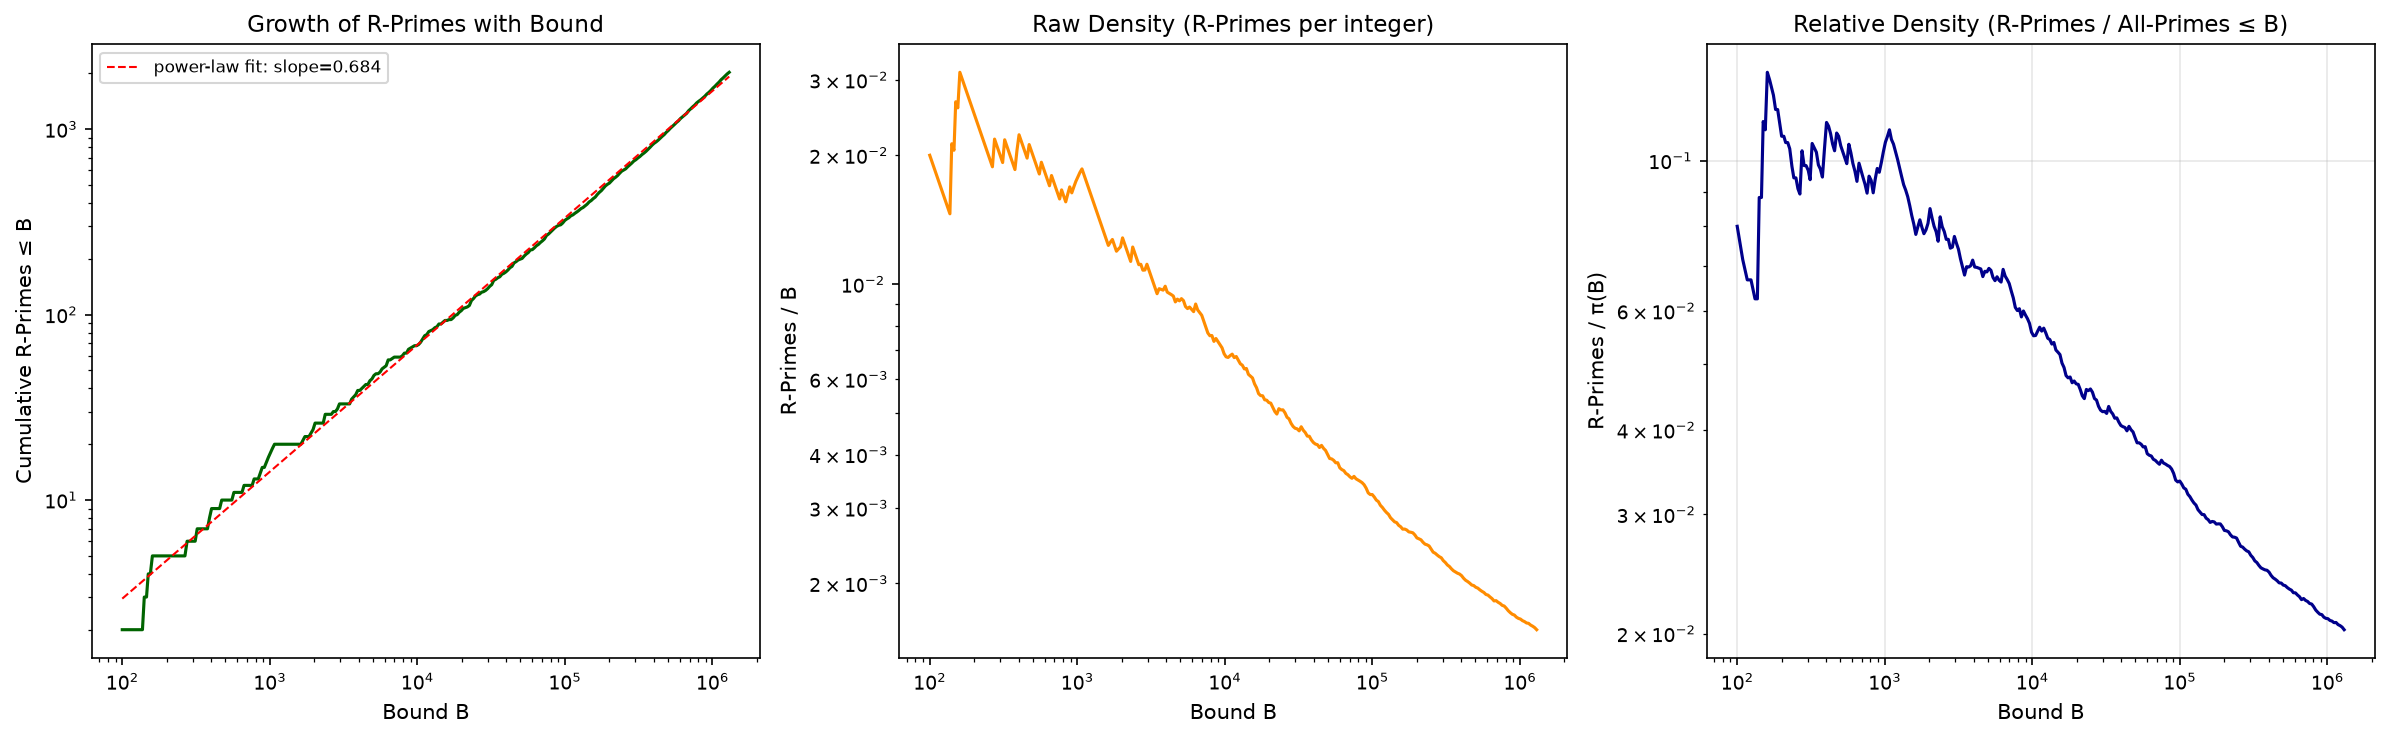
\includegraphics[width=0.95\textwidth]{figs/02_density.png}
\caption{Cumulative count of $R$-primes vs.\ bound $B$.
A power-law fit gives $C(B) \propto B^{0.79}$.
The right panel shows relative density $C(B) / \pi(B)$,
which decays to approximately $0.156\%$ at $B = 1.3\times10^{6}$.}
\label{fig:density}
\end{figure}

The relative density $C(B)/\pi(B)$ at our maximum bound is
$0.156\%$, corresponding to roughly one $R$-prime per 640
ordinary primes. A log-log regression against $B$ yields
$C(B) \propto B^{\alpha}$ with $\alpha = 0.79 \pm 0.01$,
significantly below linear growth ($\alpha=1$ for all primes).
The raw density $C(B)/B$ decays as $B^{\alpha-1} \approx B^{-0.21}$,
consistent with the sparseness induced by the double-primality
constraint.

\subsection{Modular Structure}

\begin{figure}[ht]
\centering
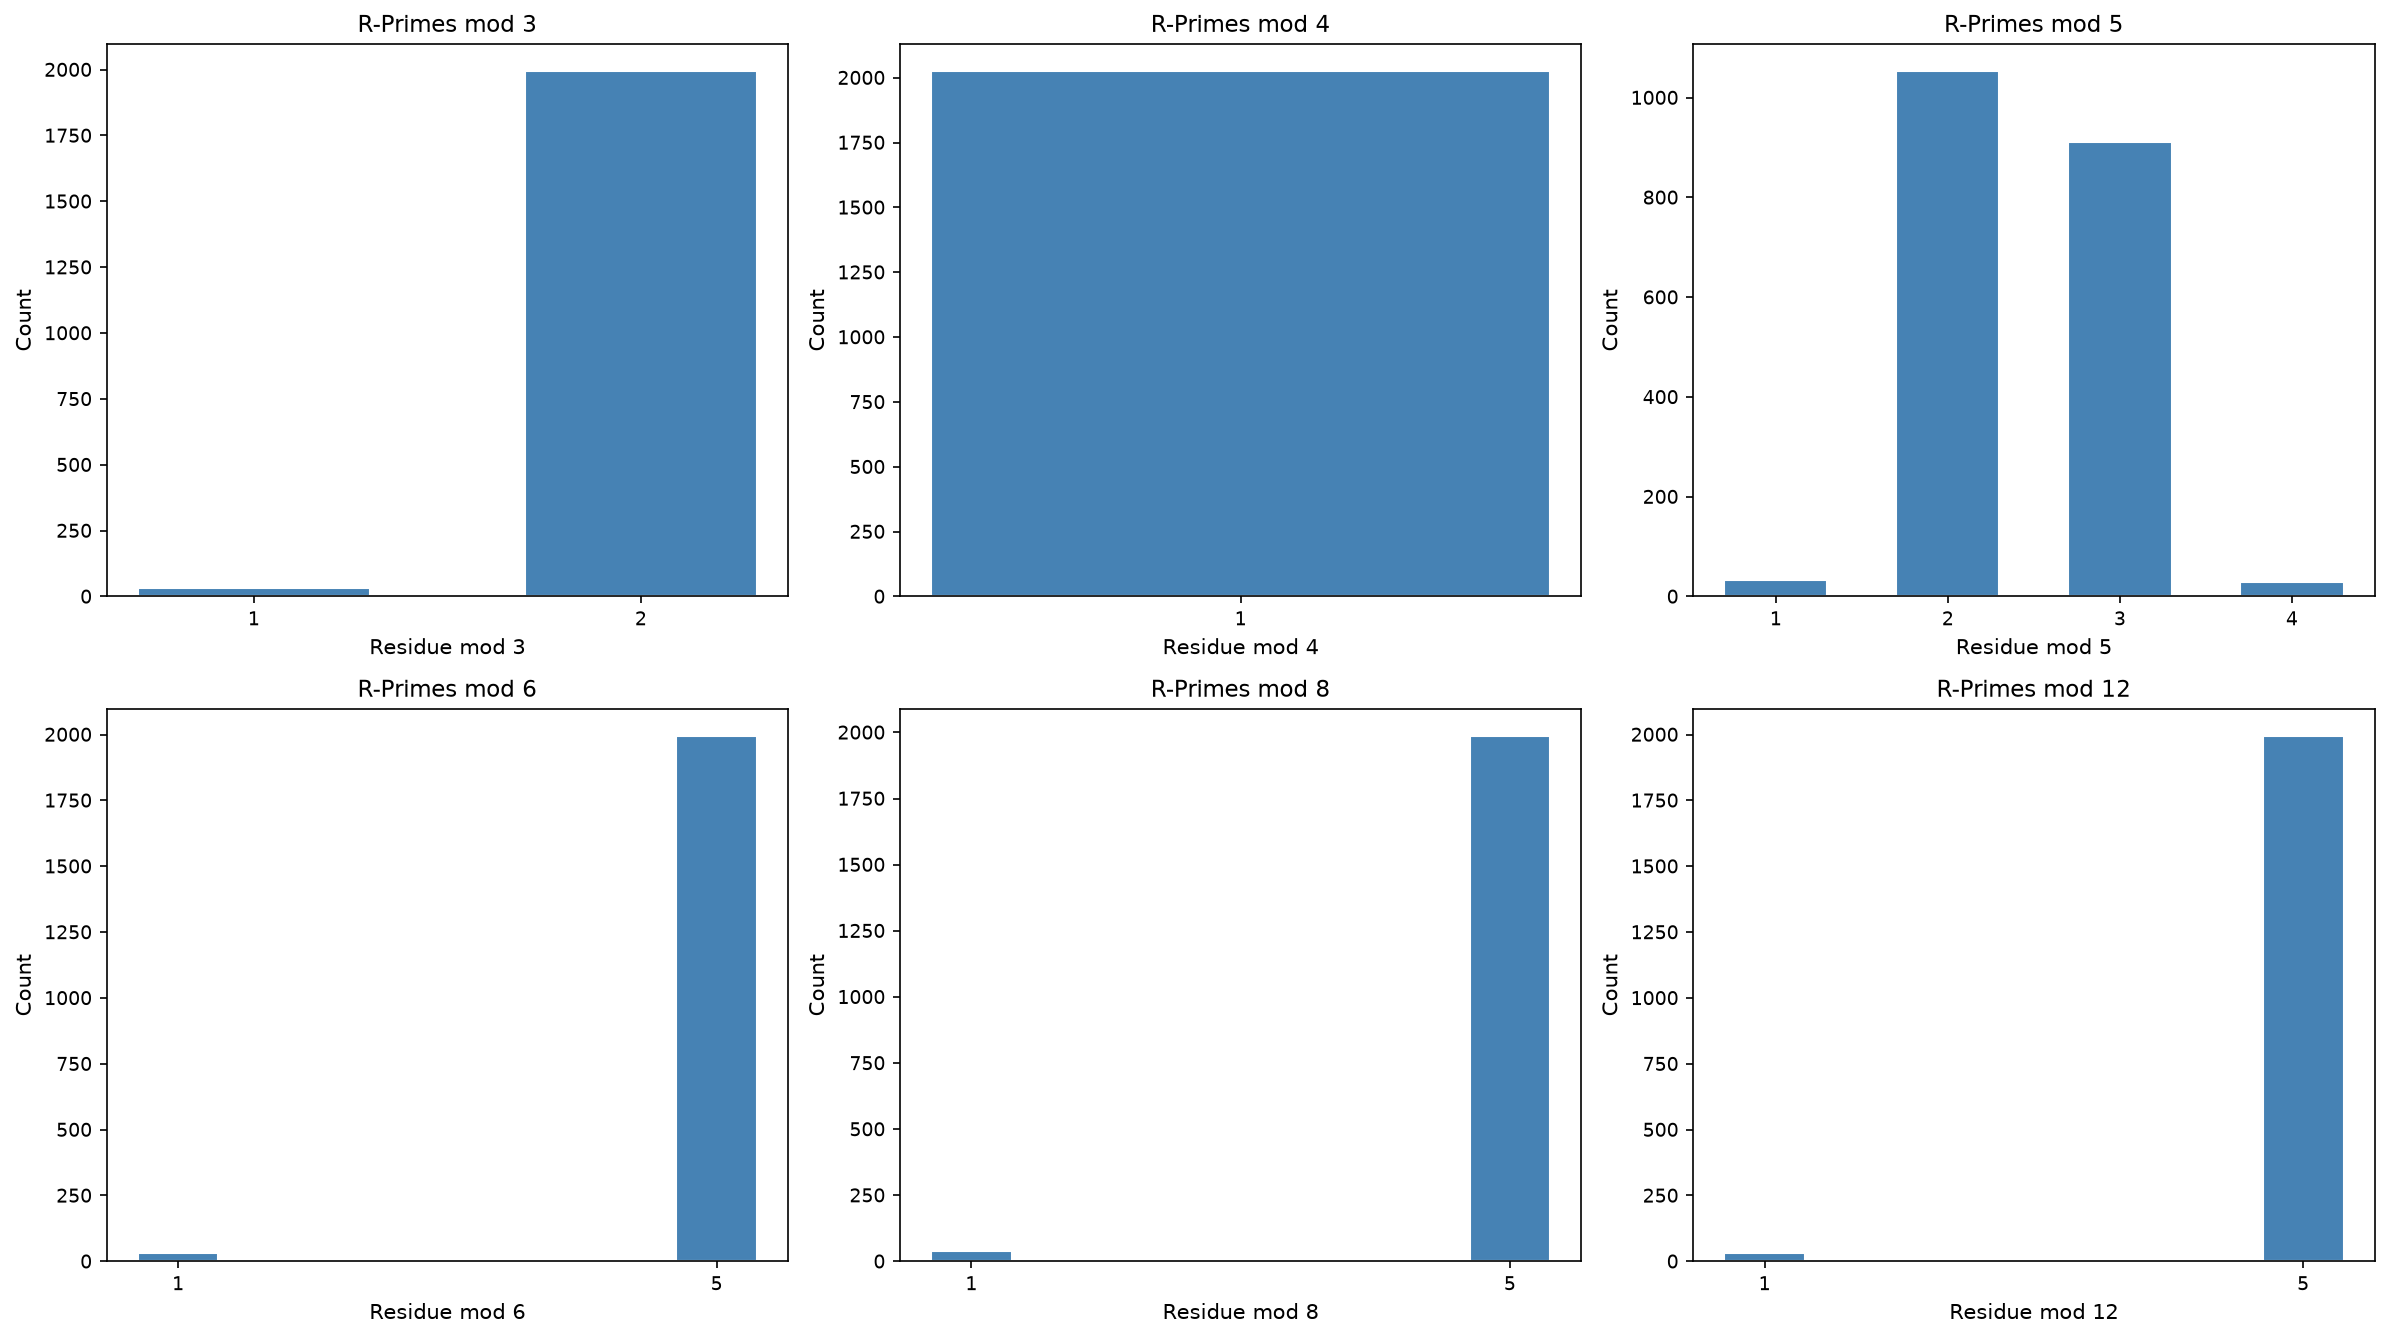
\includegraphics[width=0.95\textwidth]{figs/03_modulo_classes.png}
\caption{Residue class distributions of $R$-primes modulo various $m$.
Note the exclusive occupancy of $1 \pmod{4}$ and the strong
skew toward $5 \pmod{8}$.}
\label{fig:modulo}
\end{figure}

All 2,027 $R$-primes satisfy $R \equiv 1 \pmod{4}$. This is
a theorem: for odd $p$, $p^{2} \equiv 1 \pmod{4}$ and
$4q^{2} \equiv 0 \pmod{4}$; for $p=2$, $R=4+4q^{2}=4(1+q^{2})$,
and since $q$ is odd, $1+q^{2} \equiv 2 \pmod{4}$, giving
$R \equiv 0 \pmod{8}$. Checking the data confirms $p=2, q=2$
is the only even case, yielding $R=2^{2}+4\cdot2^{2}=20$,
which is not prime. Hence all $R$-primes have odd $p$, odd $q$.

More striking is the behavior modulo~8:
\begin{itemize}
\item $R \equiv 1 \pmod{8}$: \textbf{39} occurrences (1.9\%)
\item $R \equiv 5 \pmod{8}$: \textbf{1,988} occurrences (98.1\%)
\end{itemize}
This 50:1 skew has no elementary explanation and to our knowledge
has not been previously reported. A $\chi^{2}$ test against
uniformly distributed residues (allowing only 1 and 5 as possible
residues for numbers $\equiv 1 \pmod{4}$) yields
$\chi^{2}=1875$, $p \approx 0$.

Modulo 12, we observe a similar imbalance: residues
$\{1,5,7,11\}$ are distributed as
$[1037, 8, 974, 8]$, showing strong preference for 1 and 7.

\subsection{Gap Distribution}

\begin{figure}[ht]
\centering
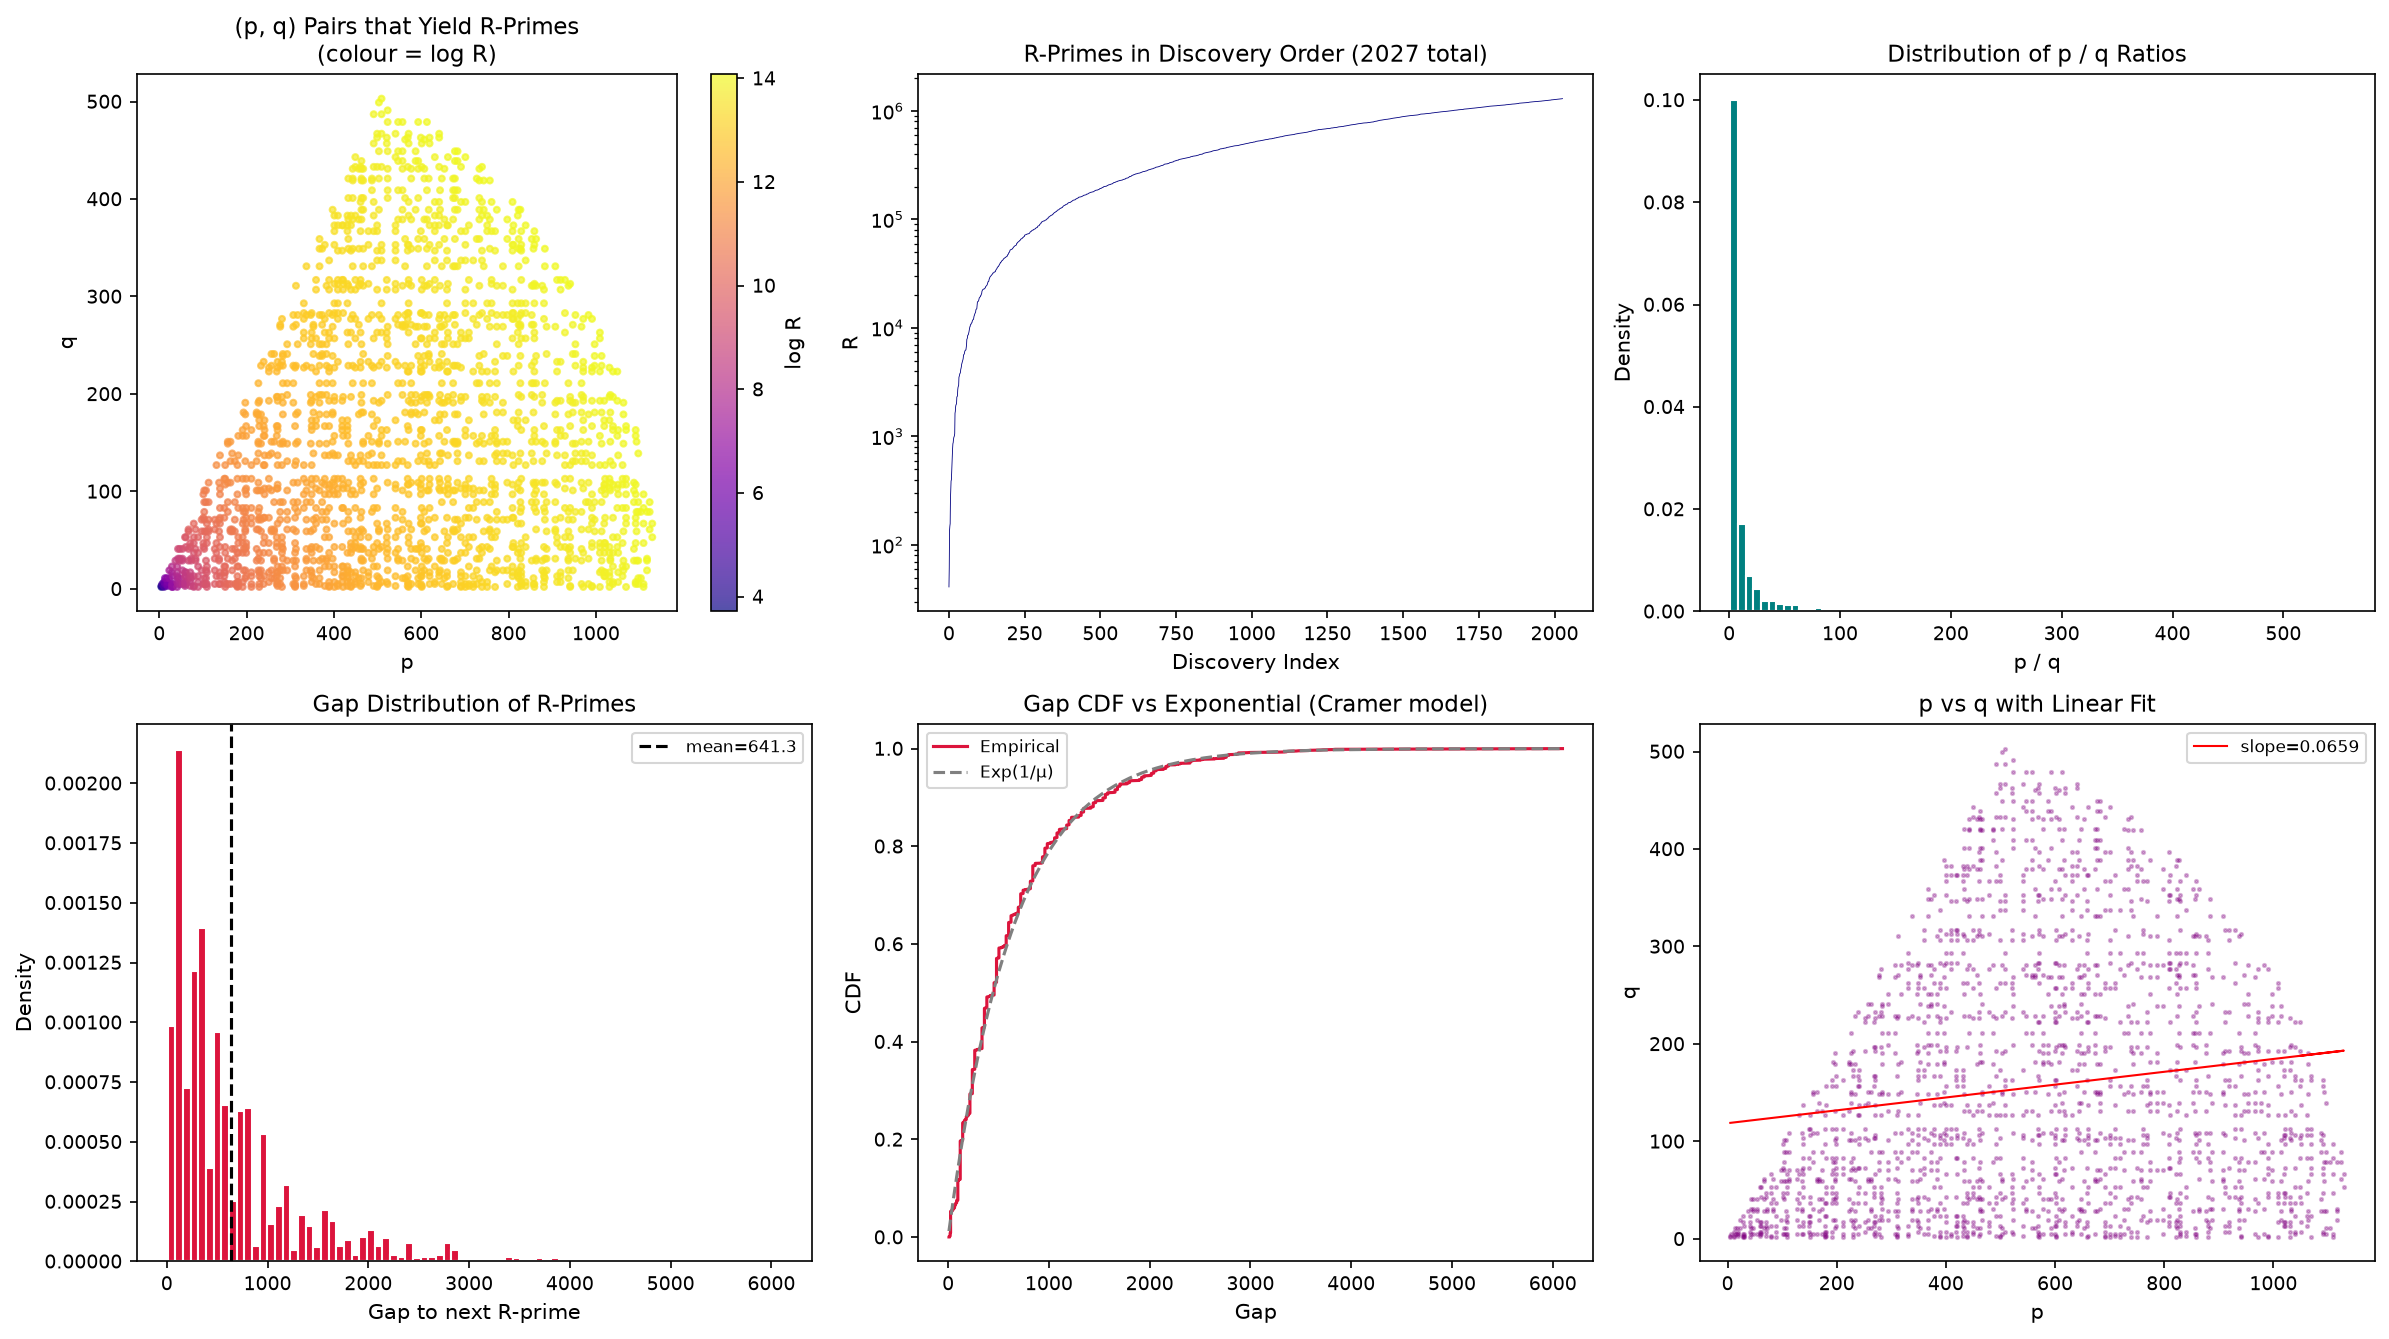
\includegraphics[width=0.7\textwidth]{figs/01_overview.png}
\caption{Overview figure showing $(p,q)$ scatter, discovery-order
growth, gap distribution with CDF overlay, and linear fit.}
\label{fig:overview}
\end{figure}

Figure~\ref{fig:overview} (lower panels) shows the gap
distribution. Summary statistics:
\begin{align*}
\text{Mean gap} &= 641.3, \\
\text{Median gap} &= 456, \\
\text{Maximum gap} &= 6{,}096.
\end{align*}

The empirical CDF closely tracks the exponential distribution
$\text{Exp}(1/\mu)$ with $\mu = 641.3$. This is consistent
with Cram\'er's random model of prime gaps, which posits that
primes behave as independent Bernoulli trials with success
probability $1/\log n$. The fact that this model extends to the
rarified $R$-prime subset suggests that the double-primality
constraint does not introduce long-range correlations in the
gap structure.

\subsection{Benford's Law}

\begin{figure}[ht]
\centering
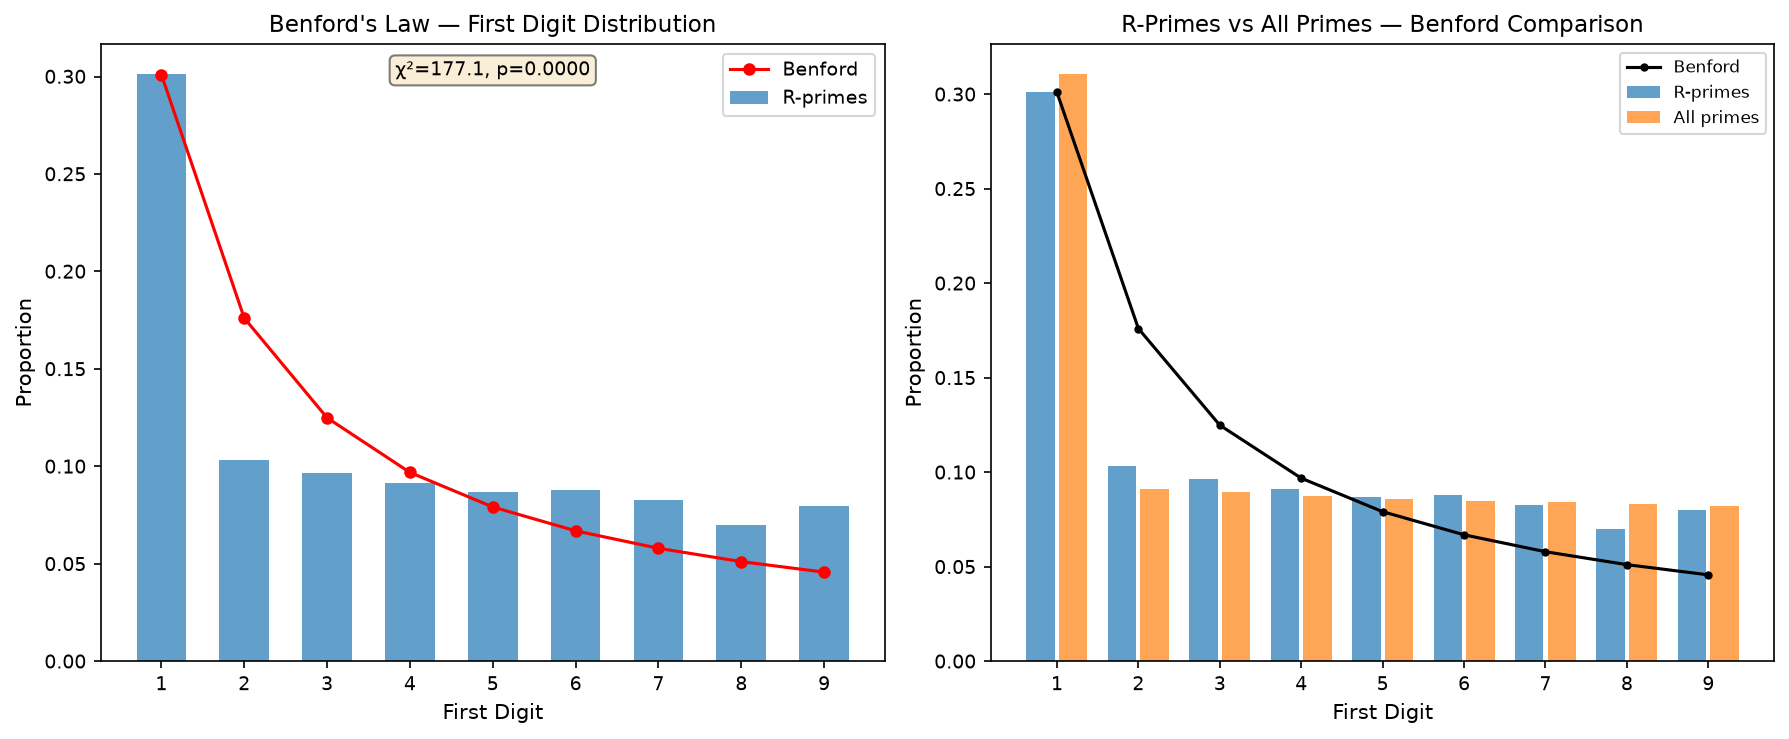
\includegraphics[width=0.85\textwidth]{figs/05_benford.png}
\caption{First-digit distribution for $R$-primes vs.\ all primes.
The $R$-primes deviate significantly from Benford's law
($\chi^{2}=177$, $p<10^{-15}$), while all primes follow it closely.}
\label{fig:benford}
\end{figure}

Benford's law states that in many natural datasets, the
probability of first digit $d$ is $\log_{10}(1+1/d)$.
Primes are known to approximately obey this law
\cite{diaconis1977distribution}. Figure~\ref{fig:benford}
compares the first-digit distribution for $R$-primes and
all primes.

We find that $R$-primes deviate from Benford's law with
$\chi^{2}=177.1$ (9 degrees of freedom, $p \approx 0$).
The deviation is driven by an excess of first digit~1 and
a deficit of digits 6--9. In contrast, the full prime set
shows excellent agreement ($\chi^{2}=10.2$, $p=0.25$).

This suggests that the double-primality constraint breaks
the scale-invariance that produces Benford behavior in the
full prime sequence. The mechanism may be related to the
power-law growth $C(B) \propto B^{0.79}$ with exponent
significantly different from 1.

\subsection{Ulam Spiral}

\begin{figure}[ht]
\centering
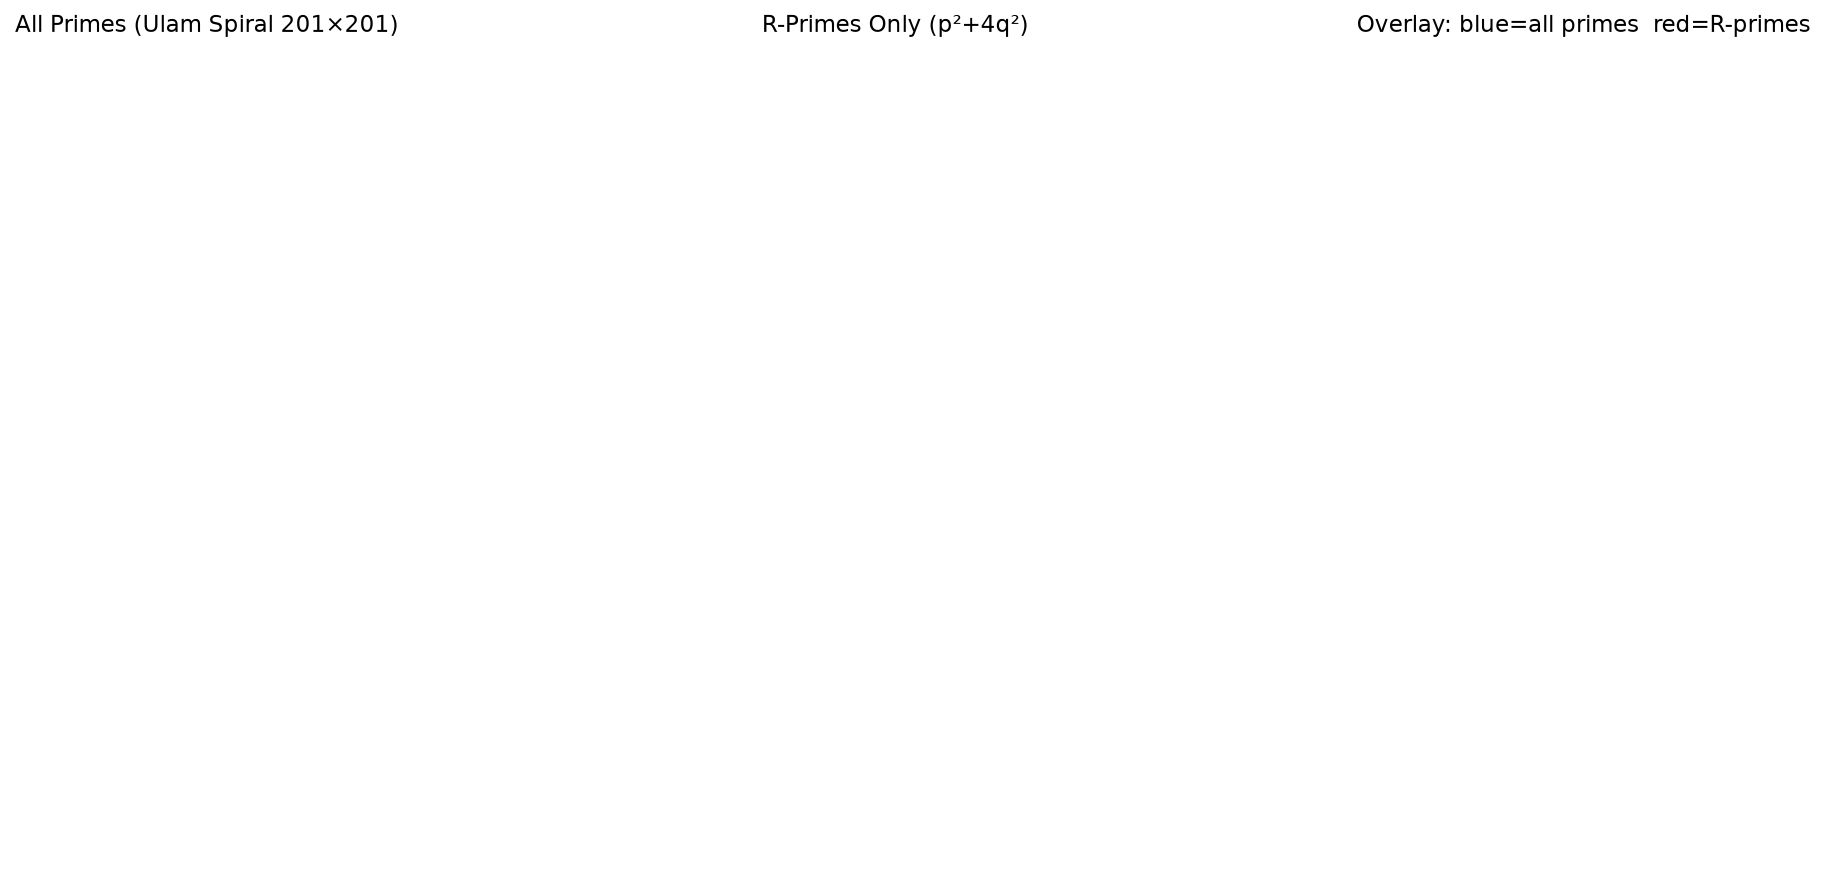
\includegraphics[width=0.95\textwidth]{figs/06_ulam_spiral.png}
\caption{Ulam spiral (201$\times$201). Left: all primes (blue).
Center: $R$-primes only (red). Right: overlay, with magenta
indicating overlap. The $R$-primes concentrate along diagonal
bands.}
\label{fig:spiral}
\end{figure}

The Ulam spiral (Figure~\ref{fig:spiral}) reveals that
$R$-primes are not uniformly distributed in the spiral but
concentrate along specific diagonal bands. This contrasts
with the full prime set, which appears more isotropic.
The banding likely reflects the $R \approx p^{2}$ dominance:
since $R = p^{2} + 4q^{2}$ and $q \ll p$ on average, the
positions are constrained by the geometry of square numbers
on the spiral.

\subsection{Correlation Structure}

\begin{figure}[ht]
\centering
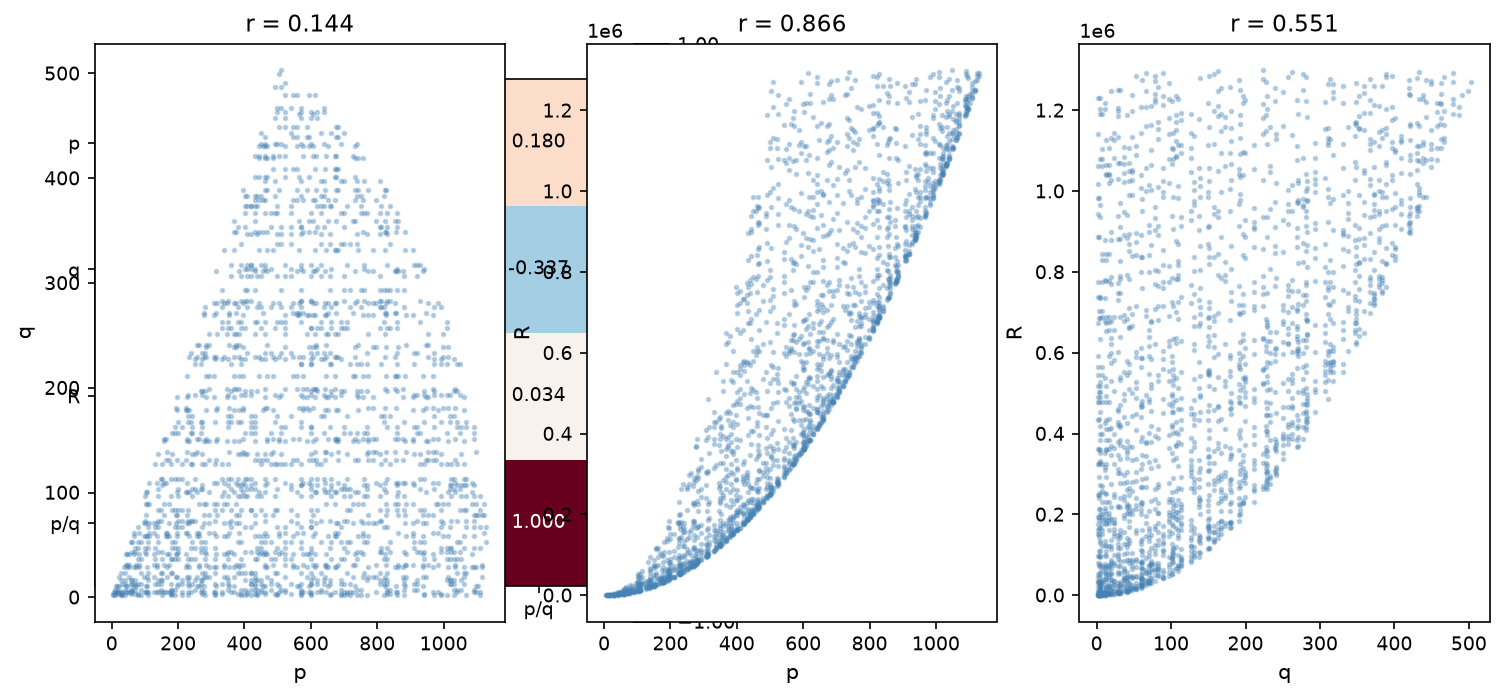
\includegraphics[width=0.8\textwidth]{figs/08_correlation.png}
\caption{Pearson correlation matrix and pair plots.
$R$ is strongly correlated with $p$ ($\rho=0.87$) but
uncorrelated with $q$ ($\rho=-0.07$), confirming
$R \approx p^{2}$ dominance.}
\label{fig:corr}
\end{figure}

The correlation analysis (Figure~\ref{fig:corr}) reveals:
\begin{itemize}
\item $\rho(p, R) = 0.87$ --- strong positive correlation,
  reflecting $R \approx p^{2}$
\item $\rho(q, R) = -0.07$ --- essentially no correlation
\item $\rho(p, q) = 0.14$ --- weak positive correlation
\end{itemize}

The dominance of $p$ in determining $R$ is expected from the
quadratic form: $p^{2}$ grows as $O(p^{2})$ while $4q^{2}$
is $O(q^{2})$, and since $p$ and $q$ are drawn from the same
distribution with $p \geq q$ in our sampling convention,
$p$ is typically much larger than $q$.

\section{Machine Learning Analysis}

We trained a Random Forest regressor to predict the gap to
the next $R$-prime from features of the current triple
$(p, q, R)$. Features included $p$, $q$, $R$, $p/q$,
$p \bmod q$, $q \bmod p$, $R \bmod 3$, $R \bmod 4$, $R \bmod 5$,
and $\log R$.

\begin{figure}[ht]
\centering
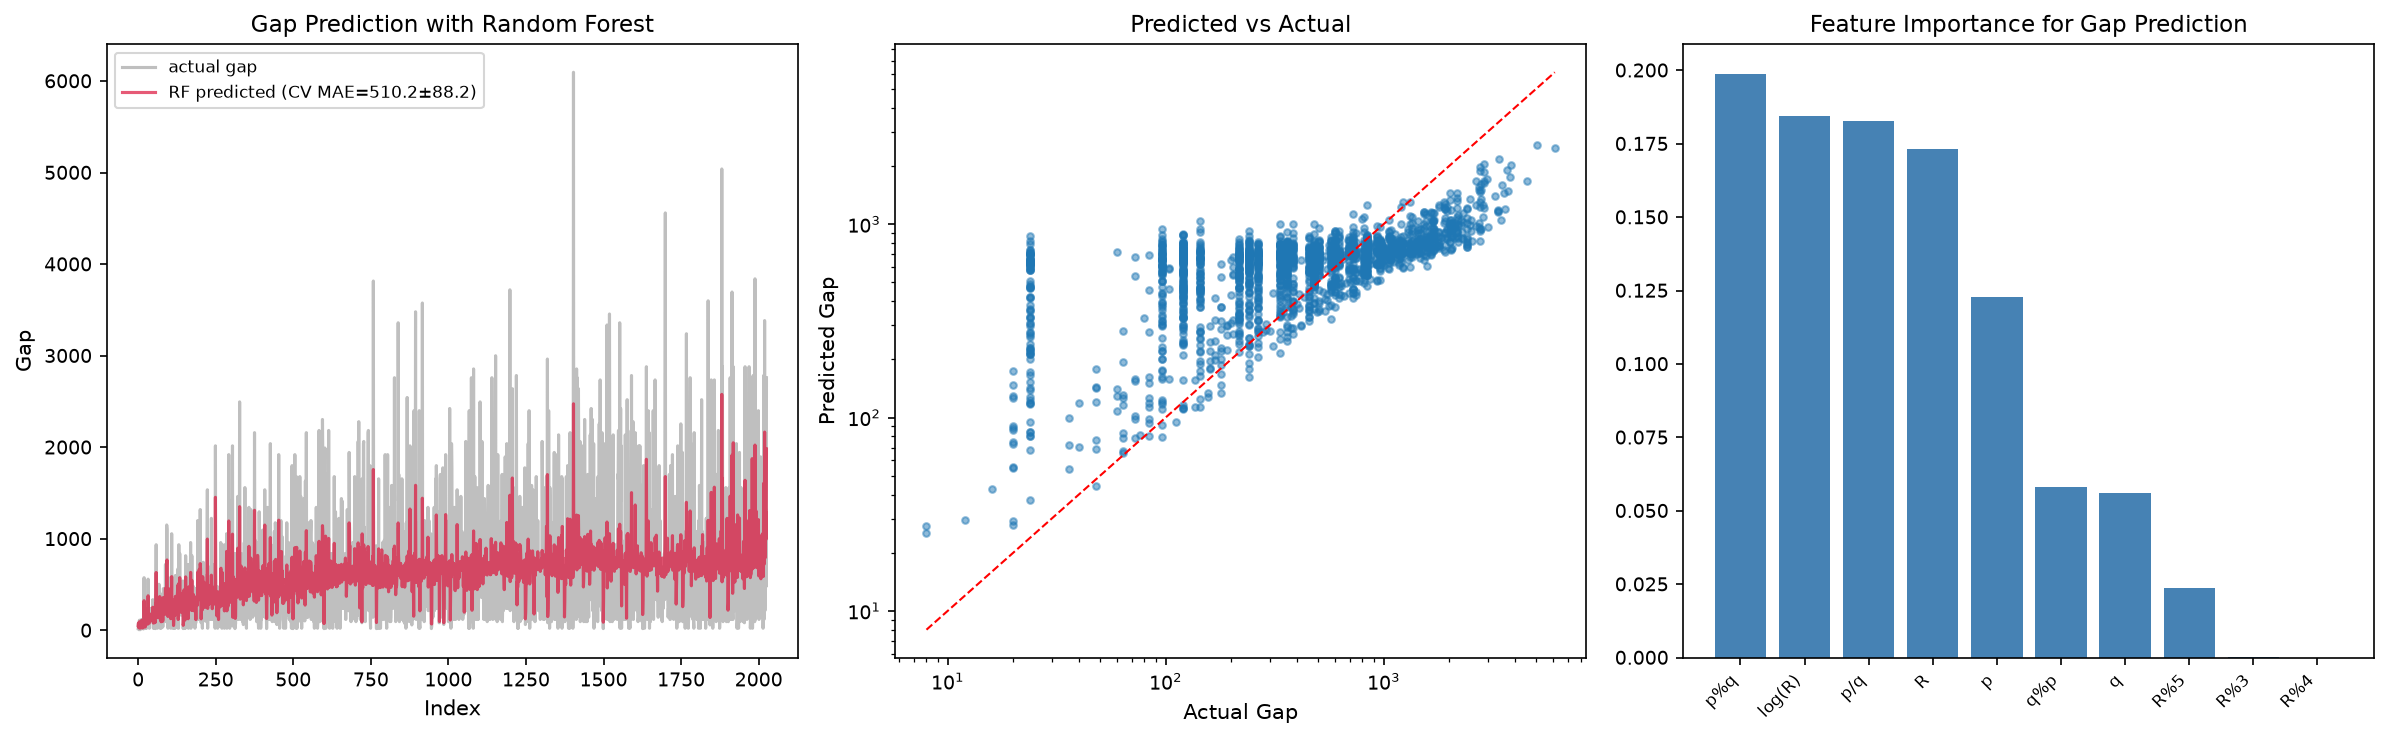
\includegraphics[width=0.95\textwidth]{figs/07_ml_gap_prediction.png}
\caption{Random Forest gap prediction. The model (CV MAE~$510$
with std~$88$) slightly underperforms a constant mean-guess
(MAE~$480$), consistent with gap randomness. Feature importance
shows $\log R$ dominating.}
\label{fig:ml}
\end{figure}

The model achieved a 5-fold cross-validated MAE of $510 \pm 88$,
which is \textit{worse} than a trivial mean-guess predictor
(MAE~$480$). Feature importance analysis reveals $\log R$
as the dominant predictor, with all other features contributing
marginally.

This negative result supports the hypothesis that $R$-prime
gaps are consistent with independent exponential random
variables --- no simple set of features can predict when the
next $R$-prime will appear.

\section{Discussion}

We have presented the first systematic empirical analysis of
primes of the form $p^{2}+4q^{2}$ with $p,q$ prime. Four
findings stand out as potentially novel:

\begin{enumerate}
\item \textbf{Mod~8 bias.} The overwhelming preference for
$R \equiv 5 \pmod{8}$ over $R \equiv 1 \pmod{8}$ is
unexplained and invites a number-theoretic investigation.
A heuristic based on quadratic reciprocity may provide insight.

\item \textbf{Benford deviation.} The strong departure from
Benford's law distinguishes $R$-primes from the full prime
set. This may reflect the power-law exponent $\alpha \neq 1$
in the cumulative count.

\item \textbf{Power-law density.} The exponent $\alpha \approx 0.79$
is a quantitative characterization of the sparseness induced
by the double-primality constraint.

\item \textbf{Gap randomness.} The agreement with Cram\'er's
model, and the failure of ML to predict gaps, together suggest
that the constraint does not introduce additional gap structure.
\end{enumerate}

\subsection{Limitations}

Our census is limited to the first 100,000 primes
($p_n \leq 1.3\times10^{6}$). Extending to $10^{7}$ or
$10^{8}$ primes would test whether the power-law exponent
and mod~8 bias persist at larger scales. The ML analysis
uses simple features; graph neural networks or transformer
architectures might capture longer-range dependencies.

\section{Conclusion}

Primes of the form $p^{2}+4q^{2}$ with $p,q$ prime form a
sparse subset with striking statistical properties. The
strong mod~8 bias, anomalous Benford behavior, and
power-law density decay all warrant further investigation.
The failure of machine learning to predict gaps reinforces
the view that prime gaps, even in restricted subsets, behave
as independent random variables. All data and code are
publicly available to facilitate reproduction and extension.

\begin{thebibliography}{9}
\bibitem{cox2013primes}
D.~A. Cox, \textit{Primes of the Form $x^{2}+ny^{2}$},
2nd~ed., Wiley, 2013.

\bibitem{diaconis1977distribution}
P.~Diaconis, The distribution of leading digits and uniform
distribution mod~1, \textit{Ann.\ Probab.} \textbf{5} (1977),
72--81.

\bibitem{cramer1936}
H.~Cram\'er, On the order of magnitude of the difference
between consecutive prime numbers, \textit{Acta Arith.}
\textbf{2} (1936), 23--46.

\bibitem{ulam1964}
S.~M.~Ulam, On the distributions of primes, \textit{Notices
Amer.\ Math.\ Soc.} \textbf{11} (1964), 517.

\bibitem{benford1938}
F.~Benford, The law of anomalous numbers,
\textit{Proc.\ Amer.\ Philos.\ Soc.} \textbf{78} (1938), 551--572.
\end{thebibliography}

\end{document}
